\subsubsection{Шаговый модуль}

Как было показано в разделе \ref{sec_feedback_control}, эффективность управления
можно повысить, если переключать фазы двигателя исходя из величины оптимальногого
при данных условиях угла коммутации. Алгоритм определения оптимального угла
коммутации описывается в разделе \ref{sec_comm_angle}.

Покажем принцип переключения активной фазы шагового двигателя на примере простого
четырёхфазного шагового двигателя. Условно процесс движения ротора шагового двигателя
можно разделить на элементарные части, состоящие из двух этапов при нормальной
работе и третьего этапа выпада из синхронизма:

\begin{enumerate}
    \item Этап движения
    \item Этап переключения
    \item Этап выпада из сихронизма
\end{enumerate}

Каждый из этих этапов имеет место в тот момент, когда ротор находится в
соответствующей зоне рассогласования векторов магнитных полей статора и ротора
(пренебрежём на данном этапе конечной скоростью нарастания тока в фазах, описанным
в разделе \ref{sec_feedback_control}).

Таким образом, решение о необходимости переключения фаз принимается на основании
анализа того, в какой зоне находится ротор двигателя в данный момент. Найдём условия,
необходимые для этого, проанализировав процесс вращения ротора двигателя в
положительном и отрицательном направлениях.

\textit{Зоной движения} будем называть зону, в которой ротор совершает движения в рамках
текущего шага, включена нужная фаза и, следовательно, перелюкчение не требуется.

\textit{Зоной переключения} будем называть зону, в которой пришло время включения
следующей фазы.

\textit{Зоной выпада из синхронизма} будем называть зону, в которую попадает ротор
двигателя в случае пропуска шагов или возникновения некоторой непредвиденной ситуации
(например, удара, отбросившего ротор назад). Так как зоны не пересекаются, но граничат
друг с другом, зону выпада из синхронизма можно определить как всю область вне зон
движения и переключения.

В соответствие с принятыми обозначениями, будем обозначать угловое положение
ротора (угловое положение вектора магнитного поля ротора) как $\theta$.
Угловое положение вектора магнитного поля статора обозначим $\phi_\textit{акт}$.


\paragraph{Движение в положительном направлении}
\begin{figure}
    \centering
    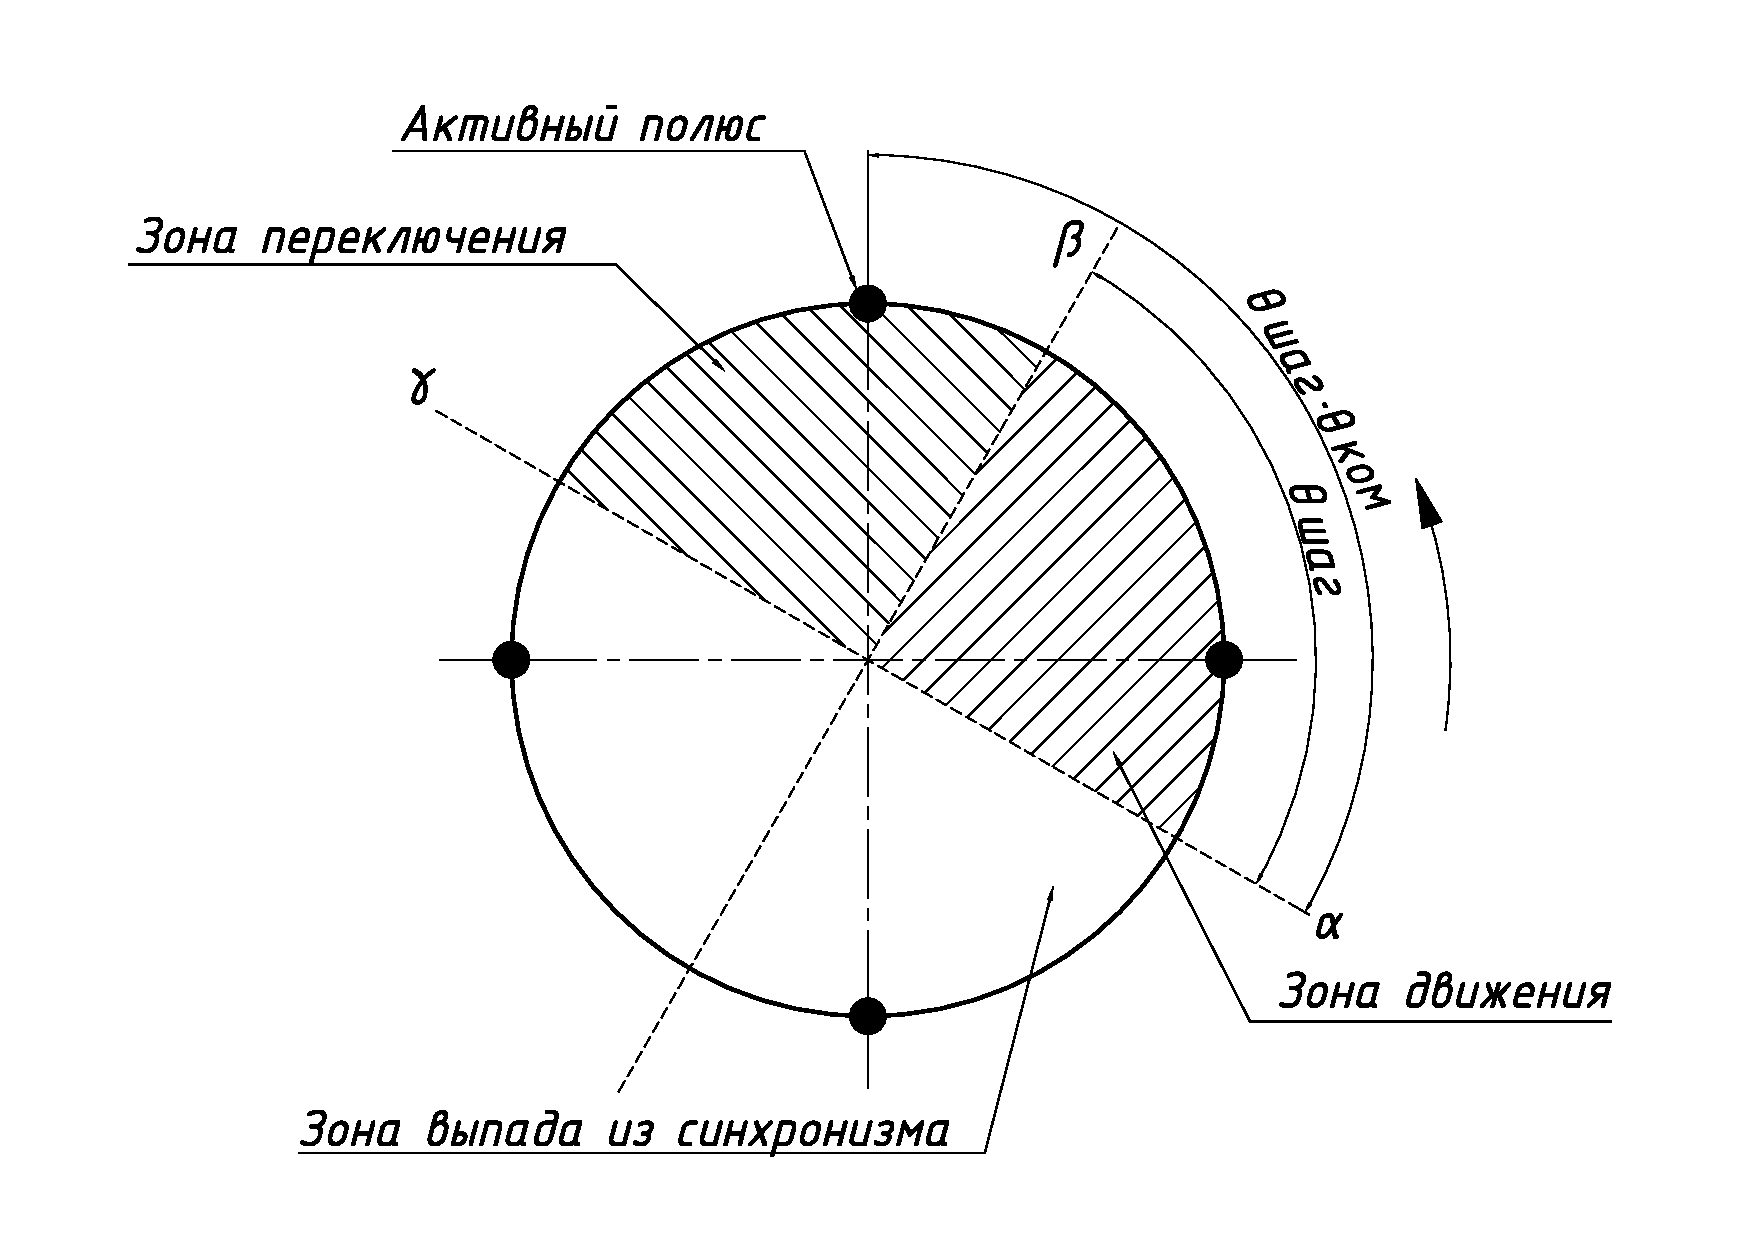
\includegraphics[width=0.7\textwidth, keepaspectratio]
                    {./src/pictures/feedback_control/pole_switch_zones_with_positive_dir}
    \caption{Зоны рассогласований магнитных векторов ротора и статора при вращении в положительном направлении}
    \label{pole_switch_zones_with_positive_dir}
\end{figure}

В зоне движения угловое положение ротора $\theta$ будет удовлетворять следующему условию:

\begin{equation}
    \label{movement_zone_posit_move_for_curr_pos}
    \begin{array}{ccccc}
        \alpha & < & \theta & < & \beta                                         \\
        \phi_\textit{акт} - \theta_\textit{ком} & < & \theta
        & < &\phi_\textit{акт} - (\theta_\textit{ком} - \theta_\textit{шаг})
    \end{array}
\end{equation}

Преобразовав это неравенство, получим выражение, описывающее границы зоны движения
в величинах рассогласования векторов магнитных полей статора и ротора:

\begin{equation}
    \label{movement_zone_posit_move_for_delta}
    \theta_\textit{ком} - \theta_\textit{шаг} < \phi_\textit{акт} - \theta
    < \theta_\textit{ком}
\end{equation}

В зоне переключения угловое положение ротора $\theta$ будет удовлетворять следующему условию:

\begin{equation}
    \label{switch_zone_posit_move_for_curr_pos}
    \begin{array}{ccccc}
        \beta & < & \theta & < & \gamma                                         \\
        \phi_\textit{акт} - (\theta_\textit{ком} - \theta_\textit{шаг}) & < & \theta
        & < &\phi_\textit{акт} - (\theta_\textit{ком} - 2\theta_\textit{шаг})
    \end{array}
\end{equation}

Преобразовав это неравенство, получим выражение, описывающее границы зоны переключения
в величинах рассогласования векторов магнитных полей статора и ротора:

\begin{equation}
    \label{switch_zone_posit_move_for_delta}
    \theta_\textit{ком} - 2\theta_\textit{шаг} < \phi_\textit{акт} - \theta
    < \theta_\textit{ком} - \theta_\textit{шаг}
\end{equation}


\paragraph{Движение в отрицательном направлении}
\begin{figure}
    \centering
    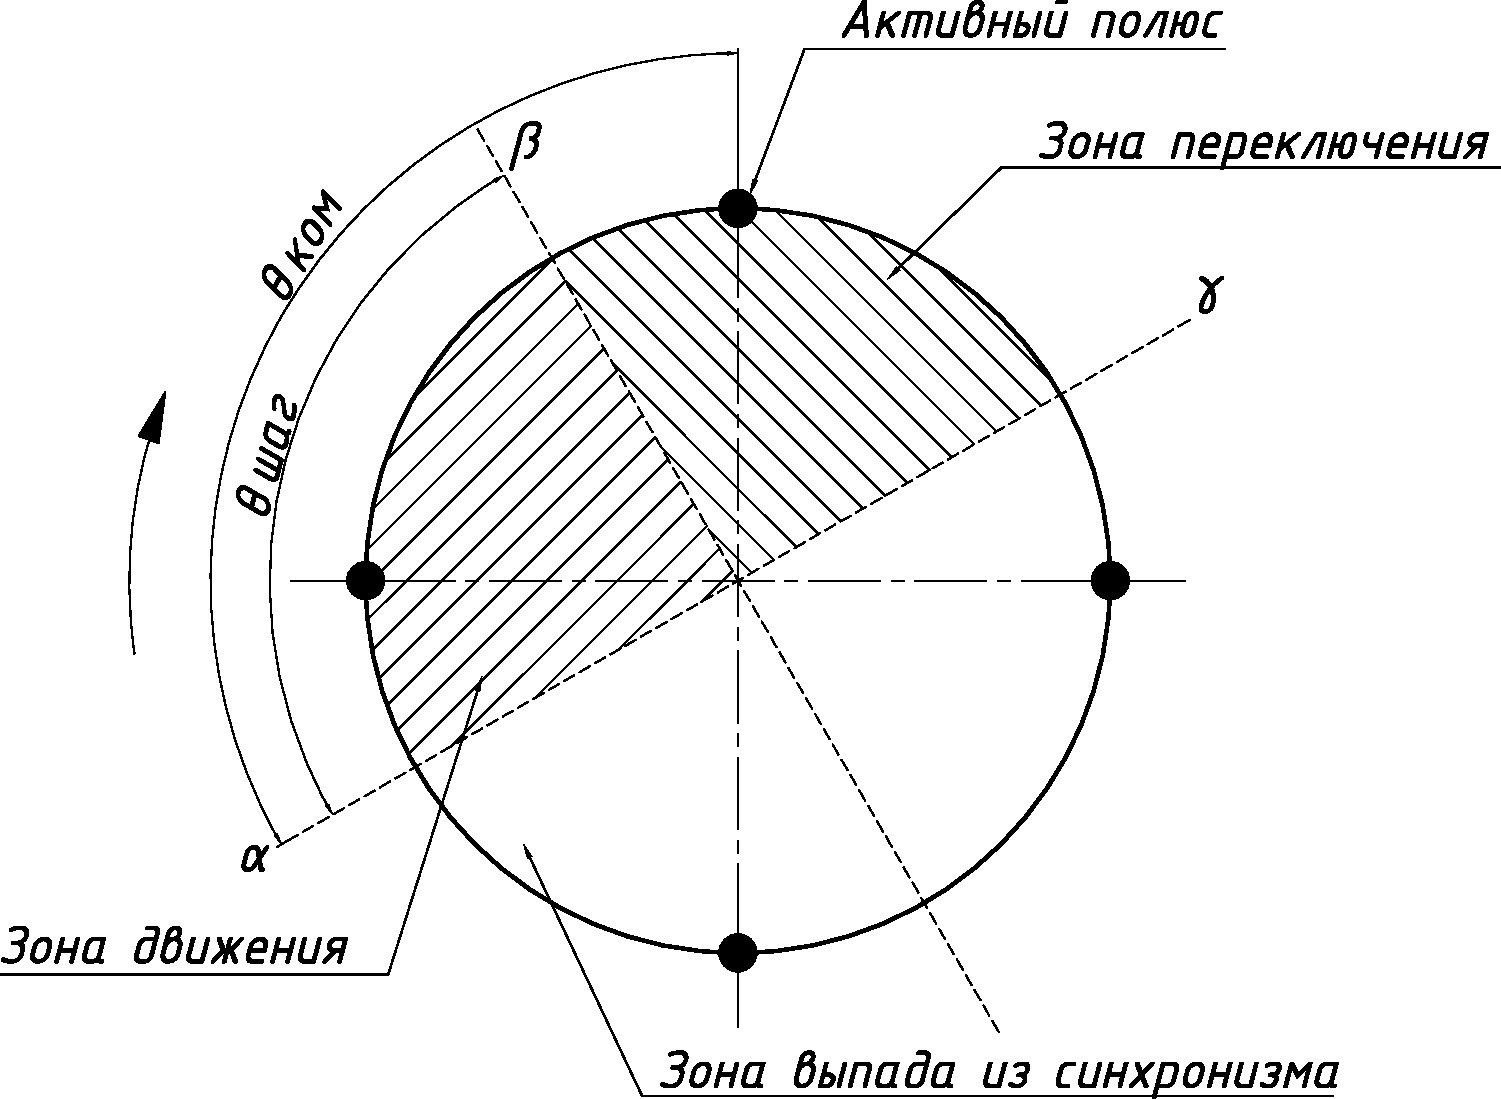
\includegraphics[width=0.7\textwidth, keepaspectratio]
                    {./src/pictures/feedback_control/pole_switch_zones_with_negative_dir}
    \caption{Зоны рассогласований магнитных векторов ротора и статора при вращении в отрицательном направлении}
    \label{pole_switch_zones_with_negative_dir}
\end{figure}

В зоне движения угловое положение ротора $\theta$ будет удовлетворять следующему условию:

\begin{equation}
    \label{movement_zone_negat_move_for_curr_pos}
    \begin{array}{ccccc}
        \beta & < & \theta & < & \alpha                                         \\
        \phi_\textit{акт} + \theta_\textit{ком} - \theta_\textit{шаг} & < & \theta
        & < &\phi_\textit{акт} + \theta_\textit{ком}
    \end{array}
\end{equation}

Преобразовав это неравенство, получим выражение, описывающее границы зоны движения
в величинах рассогласования векторов магнитных полей статора и ротора:

\begin{equation}
    \label{movement_zone_negat_move_for_delta}
    -\theta_\textit{ком} < \phi_\textit{акт} - \theta
    < \theta_\textit{шаг} - \theta_\textit{ком}
\end{equation}

В зоне переключения угловое положение ротора $\theta$ будет удовлетворять следующему условию:

\begin{equation}
    \label{switch_zone_negat_move_for_curr_pos}
    \begin{array}{ccccc}
        \gamma & < & \theta & < & \beta                                         \\
        \phi_\textit{акт} + \theta_\textit{ком} - 2\theta_\textit{шаг} & < & \theta
        & < &\phi_\textit{акт} + \theta_\textit{ком} - \theta_\textit{шаг}
    \end{array}
\end{equation}

Преобразовав это неравенство, получим выражение, описывающее границы зоны переключения
в величинах рассогласования векторов магнитных полей статора и ротора:

\begin{equation}
    \label{switch_zone_negat_move_for_delta}
    \theta_\textit{шаг} - \theta_\textit{ком} < \phi_\textit{акт} - \theta
    < 2\theta_\textit{шаг} - \theta_\textit{ком}
\end{equation}


\paragraph{Обобщение результатов}

Обозначив направление движения как $\textit{dir} = \pm 1$ и объединив формулы
для двух направлений движений, получим для зоны движения

\begin{equation}
    \label{movement_zone_for_delta}
    \theta_\textit{ком} - \theta_\textit{шаг} < dir \cdot (\phi_\textit{акт} - \theta)
    < \theta_\textit{ком}
\end{equation}

и для зоны переключения

\begin{equation}
    \label{switch_zone_for_delta}
    \theta_\textit{ком} - 2\theta_\textit{шаг} < dir \cdot (\phi_\textit{акт} - \theta)
    < \theta_\textit{ком} - \theta_\textit{шаг}
\end{equation}
